\documentclass{beamer}

%
% Choose how your presentation looks.
%
% For more themes, color themes and font themes, see:
% http://deic.uab.es/~iblanes/beamer_gallery/index_by_theme.html
%
\mode<presentation>
{
  \usetheme{default}      % or try Darmstadt, Madrid, Warsaw, ...
  \usecolortheme{default} % or try albatross, beaver, crane, ...
  \usefonttheme{default}  % or try serif, structurebold, ...
  \setbeamertemplate{navigation symbols}{}
  \setbeamertemplate{caption}[numbered]
  \setbeamertemplate{footline}[page number]
  \setbeamercolor{frametitle}{fg=white}
  \setbeamercolor{footline}{fg=black}
} 

\usepackage[english]{babel}
\usepackage[utf8x]{inputenc}
\usepackage{tikz}
\usepackage{listings}
\usepackage{courier}

\xdefinecolor{darkblue}{rgb}{0.1,0.1,0.7}
\xdefinecolor{darkorange}{rgb}{0.8,0.5,0}
\xdefinecolor{dianablue}{rgb}{0.18,0.24,0.31}
\definecolor{commentgreen}{rgb}{0,0.6,0}
\definecolor{stringmauve}{rgb}{0.58,0,0.82}

\lstset{ %
  backgroundcolor=\color{white},      % choose the background color
  basicstyle=\ttfamily\small,         % size of fonts used for the code
  breaklines=true,                    % automatic line breaking only at whitespace
  captionpos=b,                       % sets the caption-position to bottom
  commentstyle=\color{commentgreen},  % comment style
  escapeinside={\%*}{*)},             % if you want to add LaTeX within your code
  keywordstyle=\color{blue},          % keyword style
  stringstyle=\color{stringmauve},    % string literal style
  showstringspaces=false,
  showlines=true
}

\lstdefinelanguage{scala}{
  morekeywords={abstract,case,catch,class,def,%
    do,else,extends,false,final,finally,%
    for,if,implicit,import,match,mixin,%
    new,null,object,override,package,%
    private,protected,requires,return,sealed,%
    super,this,throw,trait,true,try,%
    type,val,var,while,with,yield},
  otherkeywords={=>,<-,<\%,<:,>:,\#,@},
  sensitive=true,
  morecomment=[l]{//},
  morecomment=[n]{/*}{*/},
  morestring=[b]",
  morestring=[b]',
  morestring=[b]"""
}

\title[2016-12-16-femtocode-overview]{Teraserver and Femtocode Overview}
\author{Jim Pivarski}
\institute{Princeton University -- DIANA}
\date{December 16, 2016}

\begin{document}

\logo{\pgfputat{\pgfxy(0.11, 8)}{\pgfbox[right,base]{\tikz{\filldraw[fill=dianablue, draw=none] (0 cm, 0 cm) rectangle (50 cm, 1 cm);}}}\pgfputat{\pgfxy(0.11, -0.6)}{\pgfbox[right,base]{\tikz{\filldraw[fill=dianablue, draw=none] (0 cm, 0 cm) rectangle (50 cm, 1 cm);}\includegraphics[height=0.99 cm]{diana-hep-logo.png}\tikz{\filldraw[fill=dianablue, draw=none] (0 cm, 0 cm) rectangle (4.9 cm, 1 cm);}}}}

\begin{frame}
  \titlepage
\end{frame}

\logo{\pgfputat{\pgfxy(0.11, 8)}{\pgfbox[right,base]{\tikz{\filldraw[fill=dianablue, draw=none] (0 cm, 0 cm) rectangle (50 cm, 1 cm);}\includegraphics[height=1 cm]{diana-hep-logo.png}}}}

% Uncomment these lines for an automatically generated outline.
%\begin{frame}{Outline}
%  \tableofcontents
%\end{frame}

\begin{frame}{Essential and accidental complexity}
\vspace{0.25 cm}
\textcolor{darkorange}{\bf End-user physics analysis \underline{must} consist of the following:}
\begin{description}
\item[big data pull:] probably with on-the-fly filters and transformations, given the scale of the data,
\item[manipulations:] at least plotting, but probably fitting, cross-comparisons, machine learning, etc.
\end{description}

\vfill
\textcolor{darkorange}{\bf Currently, most analyses also include:}
\begin{description}
\item[private skim:] intermediate-sized dataset with more fields than necessary.
\begin{itemize}
\item Since the big data pull takes so long, fields that {\it might} be needed are included as a hedge.
\item This makes the big data pull bigger.
\end{itemize}
\end{description}
\end{frame}

\begin{frame}{Reducing dataset size early}
\begin{center}
\only<1>{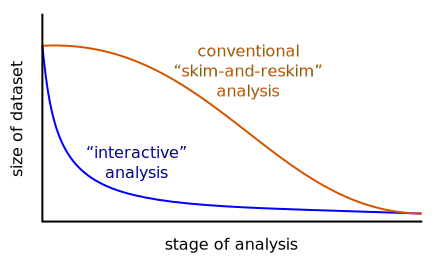
\includegraphics[width=0.8\linewidth]{pseudoplot.pdf}}
\only<2>{\includegraphics[width=0.8\linewidth]{pseudoplot2.pdf}}
\end{center}

Ideally, data should go directly from the collaboration-wide store (e.g.\ MiniAOD) into plots, fits, or machine learning algorithms, rapidly enough that there's no pressure to overstock the big data pull.
\end{frame}

\begin{frame}{Industry {\it expects} interactive analysis}

Business intelligence has traditionally been interactive; there's a race to provide interactivity with Big Data backends:

\begin{center}
\textcolor{blue}{Ibis, Impala, Kudu, Drill, \ldots}
\end{center}

all aim to yield sub-second results from terabytes or petabytes.

\vfill
\textcolor{darkorange}{\bf Shouldn't we?}
\end{frame}

\begin{frame}{Physics data are different}





\end{frame}




\end{document}
